\documentclass[]{aiaa-tc} % insert '[draft]' option to show overfull boxes

 \title{Computing Automatic Analytic Gradients on Sparse Multidisciplinary Design Problems in OpenMDAO}

\author{
  Tristan A. Hearn,%
     \thanks{Aerospace Engineer, MDAO Branch, Mail Stop 5-10, AIAA Member}
  \ Kenneth T. Moore,%
     \thanks{Senior Systems Engineer, MDAO Branch, Mail Stop 500-105, AIAA Senior Member}
  \ Justin Gray,%
     \thanks{Aerospace Engineer, MDAO Branch, Mail Stop 5-11, AIAA Member}
   \\
  {\normalsize\itshape
  NASA Glenn Research Center, Cleveland, OH}  \\
  John T. Hwang,%
  \thanks{Ph.D. Candidate, Department of Aerospace Engineering, AIAA Student Member}
  \ Joaquim R. R. A. Martins%
  \thanks{Associate Professor, Department of Aerospace Engineering, AIAA Associate Fellow}
  \\
  {\normalsize\itshape
   University of Michigan, Ann Arbor, Michigan, 48109, United States}
}

\AIAAconference{Multidisciplinary Design Optimization Specialist Conference}
\AIAAcopyright{\AIAAcopyrightD{2012}}


% Define commands to assure consistent treatment throughout document
\newcommand{\eqnref}[1]{(\ref{#1})}
\newcommand{\class}[1]{\texttt{#1}}
\newcommand{\package}[1]{\texttt{#1}}
\newcommand{\file}[1]{\texttt{#1}}
\newcommand{\BibTeX}{\textsc{Bib}\TeX}

\setlength{\abovecaptionskip}{0pt}
\setlength{\belowcaptionskip}{0pt}

\usepackage{setspace}

\usepackage{graphicx}
\usepackage{wrapfig}
\usepackage{caption}
\usepackage{amsmath}
\usepackage{lscape}
\usepackage{hyperref}
\usepackage{minted}
\usepackage{color}
\usepackage{appendix}
\usepackage[section]{placeins}

\newcommand{\txt}{\textrm}


\captionsetup[figure]{margin=5pt,font=small,labelfont=bf,textfont=bf,justification=justified,}
%\captionsetup[wrapfigure]{margin=5pt,font=small,labelfont=bf,justification=justified,singlelinecheck=off}
\captionsetup[table]{margin=5pt,font=small,labelfont=bf,textfont=bf,justification=justified,position=top}

\bibliographystyle{aiaa}

\usepackage{lettrine}
\usepackage{verbatim}

\begin{document}

  \maketitle

  \begin{abstract}

  \end{abstract}

  \section{Introduction (Justin)}

    Gradient based optimization with analytic gradients is an effective tool for solving problems
    with large design spaces. It has been applied widely for aerodynamic shape optimization \cite{Liou2010,palacios2012adjoint}
    and structural optimization\cite{Kennedy:2013:TACS, Venkataraman:2004:SOC, Adelman:1986:structure-sensitivity}.
    In order to apply these methods to multidisciplinary problems, system level derivatives must be
    constructed by combining the partial derivatives from each discipline using the Global Sensitivity
    Equations\cite{Sobieski1990}. This technique has been applied commonly to coupled
    aero-structural design optimization of aircraft wings\cite{Kenway2012c, Haghighat2012} and is applicable to
    other coupled design problems such as aero-accoustic design\cite{economon2012coupled}.Extending these
    gradient based techniques to more complex problem formulations has proved difficult. When
    design problems grow to include 10's of disciplines, it becomes increasingly difficult to construct the
    necessary derivatives. Even assuming all of the disciplines could provide analytic partial derivatives,
    the construction of the system level derivatives is heavily dependent on the structure of the data passing
    between disciplines. Manual implementations for these problems are time consuming and discourage modifications
    to the problem formulation in the future. Moore developed a method for automatically assembling the system
    level derivatives based on the data-dependency graph of a given problem formulation\cite{openmdao_derivatives}.
    In addition to allowing greater flexibility in the problem formulation, a key feature of this graph-based approach, was the efficient
    handling of sparse problem formulations. By traversing the graph from design variables to quantities of interest,
    it was possible to consider only the subset of variables that were relevant to a specific system level gradient thus
    making gradient computations more efficient.

    Although Moore's work demonstrated that a framework could compute system level derivatives for arbitrary
    problem setups, it required components to provide a full Jacobian matrix, which it assembled into
    complete system level Jacobian matrix.  This made it unsuitable for usage with
    high-fidelity tools, since they often times had far too many variables to allow assembling a full Jacobian.
    Martins and Hwang developed an alternative, graph-free, method for computing automatic system
    level sensitivities which used a global design variable vector\cite{Martins2012}.
    In a later work they added a matrix-free solver algorithm to their method that solved issue with full Jacobians from
    Moore's implementation. They demonstrated the effectiveness of their method on a design optimization of a small satellite
    with over 25,000 design variables and over 1 million state variables\cite{CADRE2012}. Despite its success,
    the global-vector based approach required all the variables from the system model be
    included when solving for system level derivatives. This prevented Martins and Hwang's method
    from taking advantage of sparsity in the problem formulation and resulted in a less efficient gradient solving step.
    As a result, over 90\% of the compute during convergence time was spent solving a linear system for the system
    level derivatives.

    This work combined the graph-based approach taken by Moore with the matrix-free solution algorithm
    developed by Martins and Hwang to efficiently compute derivatives for sparse, large-scale engineering
    design problems. The original small satellite design problem was re-run using the new method and
    a dramatic increase in efficiency was demonstrated. A second design optimization on a wind turbine was
    also performed. This problem had a more complex structure with stronger multidisciplinary couplings as well as a
    mixture of analytic and finite difference gradients.

  \section{Unfied Derivatives Computations (John)}
    Short summary of the unified derivatives method and it's implications for forward or adjoint derivatives.


  \section{Dependency Graph (Ken/Justin)}

    In Moore's original work on computing derivatives from a dependency graph, he employed
    a discipline based dependency graph, with a node for each discipline and edges describing
    dependency between the nodes. A path finding algorithm, from the NetworkX library\cite{hagberg-2008-exploring},
    computed the relevant set of disciplines for a given derivative. Although this took advantage of sparsity at
    one level, by excluding any disciplines that don't directly contribute, it can't handle a second level of sparsity
    within the relevant disciplines. Even if a given discipline is relevant, some of its variables may still not be
    because they don't directly affect the quantities of interest. Pate et. al. proposed an alternative dependency graph
    structure that addressed this problem\cite{graph_problem2013}. Each discipline and all its inputs and outputs are
    represented by nodes with directed edges between them describing their dependencies on each other.
    Figure \ref{fig:sellar_graph} shows a sample graph for the Sellar Problem \cite{AIAA:sellar}
    given in eqn. \ref{eqn:sellar_formulation}.

    \begin{align}
        \txt{given} & \ \ y_1 = D_1(x_1,y_2,z_1,z_2) \notag
        \\      & \ \ y_2 = D_2(y_1,z_1,z_2) \notag
        \\\txt{min.} &\ \ F(x_1,y_1,y_2,z_2) \notag
        \\\txt{w.r.t.} & \ \ x_1,y_1,y_2,z_1,z_2 \notag
        \\\txt{s.t.} & \ \ G_1(y_1) \geq 0 \notag
        \\     & \ \ G_2(y_2) \geq 0
        \label{eqn:sellar_formulation}
    \end{align}

    \begin{figure}[!htb]\begin{center}
      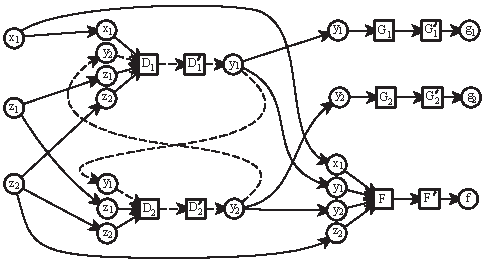
\includegraphics[width=.8\textwidth]{images/sellar_cycles}
      \caption{ Dependency graph for the Sellar problem. \label{fig:sellar_graph}}
    \end{center}\end{figure}

    In the original graph syntax, a single node is given for every variable. This graph contains all the 
    necessary information to take full advantage of problem sparsity, but suffers from one potential 
    weakness. For a problem with millions of state variables, like aerodynamic shape optimization, 
    the graph would get very large and would be inefficient to operate on. To address this issue 
    related variables, such as arrays, can be aggregated into a single node to represent the 
    overall variable. If any specific sub-variable is referenced (e.g., some slice of an array). 
    Figure \ref{fig:subvars} shows how the sub-variable nodes relate to their parent variables. Here,
    both outputs A.x and A.y are array variables. The full array A.x is connected to 
    B.x while a single element of A.y is connected to the scalar B.z.

    \begin{figure}[!htb]\begin{center}
      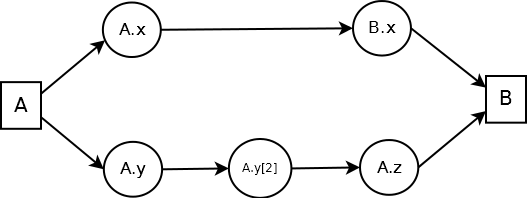
\includegraphics[width=.8\textwidth]{images/Graph1}
      \caption{ Example graph with child nodes for sub-variables \label{fig:subvars}}
    \end{center}\end{figure}

    By using the sub-variable nodes, the computational advantages of problem sparsity are retained. For example,
    consider $\frac{\partial B.z}{\partial A.y}$ from Fig. \ref{fig:subvars}. Given the graph, we know that
    this derivative will be sparse, with only $A.y[2]$ having non-zero values as in eqn.  \ref{eqn:sparse_gradient}. 

    \begin{equation}
        \frac{\partial B.z}{\partial A.y} =
        \begin{bmatrix}
            0 \\
            0 \\
            \frac{\partial B.z}{\partial A.y[2]} \\
            \vdots \\
            0 \\
        \end{bmatrix}
        \label{eqn:sparse_gradient}
    \end{equation}

    When solving for derivatives, without the sub-var node, you would need to include all the 
    elements of the $A.y$ array in the linear system for derivatives calculations. 
    With the sub-var node, only the single relevant value from the array needs to be included. 
    By representing hierarchical data as a single node, the overall size of the graph 
    remains manageable, and the sub-var nodes are used to preserve the benefits of sparsity. 


    \subsection{Graph Traversal Determining Relevance}
        
        OpenMDAO can calculate a gradient between any set of input and output nodes in the
        dependency graph by setting up the appropriate linear system. The size of the linear system
        is determined by the number of variables being considered, which means that the linear 
        system can get very large. OpenMDAO is able to achieve significant reductions in the 
        size of the linear system by traversing the dependency graph to find the sub-set of relevant variables.
        For example, consider the notional graph in Fig. \ref{fig:graph2}. Considering $\frac{\partial Obj}{\partial param}$, 
        the relevant components variables and components are highlighted. Only Components 1, 3, and 5 are needed, 
        and furthermore only $C3.a$ is needed from Component 3. 

        \begin{figure}[!htb]\begin{center}
          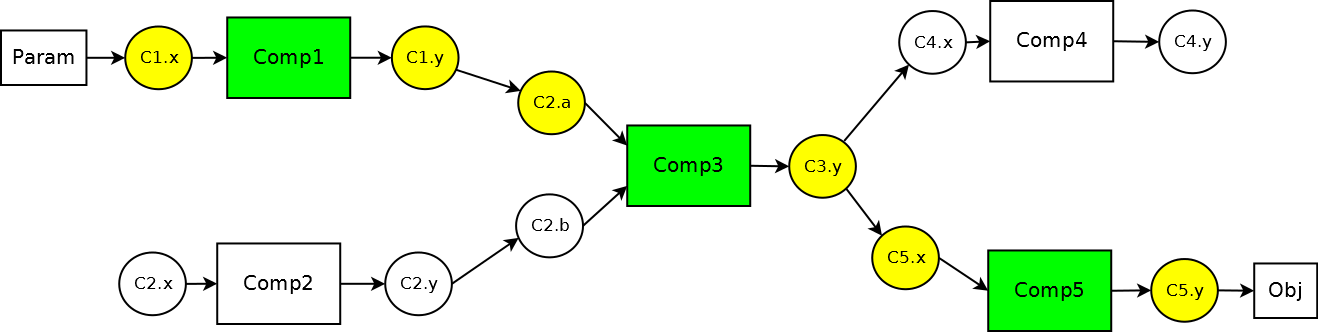
\includegraphics[width=.8\textwidth]{images/Graph2}
          \caption{ The reduced graph for the derivatives calculation includes Comps 1, 3, 
          and 5 with their interconnecting variables. \label{fig:graph2}}
        \end{center}\end{figure}

        A sub-graph like the one in Fig. \ref{fig:graph2} can be found that gives
        the minimum relevant set of components and variables necessary to solve for a specific 
        gradient. 
        
        
    \subsection{Cycle Detection and Usage}
        Pate et. al indicate that within a dependency graph, the presence of cycles indicates coupling between
        the components in the cycle \cite{graph_problem2013}. A cycle can consist of two or more components, and
        one component may be part of more than one cycle.

        In formal terms, cycles exist in a graph when a group of nodes are strongly connected. The NetworkX package
        provides an implementation of Tarjans algorithm for finding sets of strongly connected
        components\cite{tarjan1972depth,nuutila1994finding}. Once found, the presence of these cycles
        have an impact on how any given model is solved. Firstly during normal execution, these cycles
        need to be converged with a numerical solver such as Gauss-Seidel or Newton based. 
        In addition these cycles need to be accounted for when solving for the gradients 


    \section{API for Specifying Discipline Derivatives (Tristan)}

        OpenMDAO supports calculating derivatives in two ways: direct and adjoint. The direct method performs
        one linear solve for each design variable. The adjoint method performs one linear solve per each objective
        and constraints. Hence, if you have more design variables than quantities of interest (as if often the case),
        the adjoint method will require far fewer solves of the linear system. If you have fewer design variables then
        objectives and constraints the forward mode is preferable.

        OpenMDAO allows users to specify analytic derivatives of components by declaring one or more of the following three
        methods:

        \begin{itemize}
            \item provideJ(ins, outs, Jacobian)
            \item apply\_deriv(input\_vector, result\_vector)
            \item apply\_derivT(input\_vector, result\_vector)
        \end{itemize}

        The provideJ method is the simplest method to implement, and also the most flexible. The user simply gives the framework the
        Jacobian and the order of the columns and rows in that Jacobian. With that information, OpenMDAO can automatically
        implement either the forward or adjoint derivatives methods. This flexibility comes with some computational cost however.
        Although at the overall system level the Jacobian is provided as a linear operator, that linear operator is built out
        of the set of component Jacobians which are all stored in memory. If your component has relatively few inputs and outputs
        (on the order of 10's), then this cost is not likely to be significant. However, as the scale of the components grows,
        the other two functions will offer better efficiency.

        The two methods apply\_deriv and apply\_derivT implement Jacobian linear operators at
        the component level for the direct and adjoint methods respectively. So the user must provide both if they
        want the component to be able to operate in both forward and adjoint modes. If the user prefers one method over
        the other, they can choose to only implement one or the other. When both methods are present OpenMDAO will
        attempt to make an intelligent choice about whether to use the forward or adjoint method based on the number
        of variables vs objectives and constraints.



    \section{Small Satellite Design Problem (Tristan)}

    CADRE (Cubesat investigating Atmospheric Density Response to Extreme driving)
    is a mission funded by the National Science Foundation to study the
    response of the thermosphere to auroral phenomena\cite{cutler2011cubesat}. 
    The small satellite design problem optimizes the design of a cubsat for the CADRE mission. 
    This problem was originally implemented and solved by Hwang et. al\cite{CADRE2012} using 
    Martins and Hwang's matrix-free gradient strategy. The analysis models the interaction of several 
    disciplines (attitude control, communications, power and energy storage system, thermal dynamics, craft orbital 
    dynamics, and sun-earth position) over the course of a one year mission. Specifically, 
    the system is modeled over the course of six separate half-days of operation, computed at conditions
    1, 3, 5, 7, 9, and 11 months after launch. The goal was to balance performance under diverse conditions (such as relative 
    location of the sun, etc.) seen over the course of the mission.

    \subsection{Problem Formulation}

    \begin{align}
        \\\txt{max.} &\ \ \sum_{i=1}^6 Data_i \notag
        \\\txt{w.r.t.} & \ \ 0 \le I_{setpt} \le 4 \notag
        \\     & \ \ 0 \le P_{comm} \le 25 \notag
        \\     & \ \ 0 \le cellInstd \le 1 \notag
        \\     & \ \ 0 \le finAngle \le \pi/2 \notag
        \\     & \ \ 0 \le antAngle \le \pi \notag
        \\     & \ \ 0.2 \le iSOC \le 1 \notag
        \\\txt{s.t.} & \ \ I_{bat} - 5 \le 0 \notag
        \\     & \ \ -10 - I_{bat} \le 0 \notag
        \\     & \ \ 0.2 - SOC \le 0 \notag
        \\     & \ \ SOC - 1 \le 0 \notag
        \\     & \ \ fSOC - iSOC = 0 \notag
        \label{eqn:cadre_formulation}
    \end{align}

    The objective of the optimization is to maximize the total amount of data transmitted to the ground 
    station (Ann Arbor, MI) over these six design points. There are six 7 design varibles listed in Eqn. \ref{eqn:sellar_formulation}.
    3 of them, $\gamma$, $I_{setpt}$, and $P_{comm}$, are arrays of time varying schedules for the attitude, 
    solar panel current, and communications power respectively. The remaining 4, $cellInstd$, $finAngle$, $antAngle$, $iSOC$, 
    are all physical design variables of the satellite. All together there are 25,292 design variables. 
    The 5 constraints for the problem relate to the battery charge rate, battery discharge rate, 
    minimum battery capacity, maximum battery capacity, and a battery state-of-charge periodicity 
    constraint. Each constraint is a length 6 vector with a value representing each of the 6 different 
    orbits, yielding a total of 30 constraints. Since the problem has significantly more design 
    variables than it does objectives and constraints, the problem was solved using adjoint gradients. 

    \begin{figure}[!htbp]
        \centering
        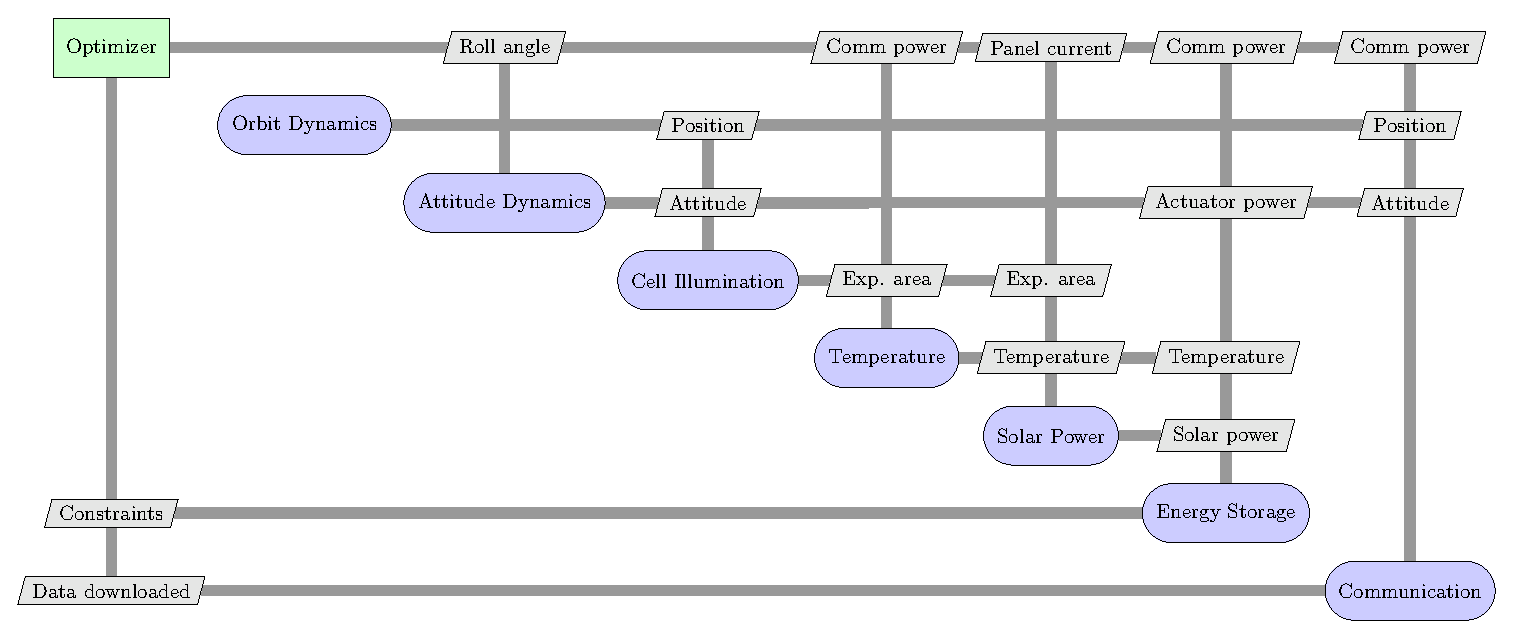
\includegraphics[width=0.95\textwidth]{images/cadre_xdsm}
        \caption{XDSM diagram showing the general structure of the small satellite design problem}
        \label{fig:cadre_xdsm}
    \end{figure}

    Overall the problem can be broken down into 7 distinct disciplines: orbit dynamics, attitude dynamics, cell illumination, 
    temperature, solar power, energy storage, and communication. Figure \ref{fig:cadre_xdsm} shows how each of the disciplines
    relate to each other in the optimization problem. The actual implementation of the problem further 
    subdivided most of the disciplines into smaller sub-disciplines. The true component level dependency 
    graph, given in Fig. \ref{fig:cadre_graph}, has 39 different components. The full graph, including all variable and 
    sub-variable nodes, is omitted for visual clarity. 

    From a problem structure standpoint, this problem has three significant features. Firstly, the large number of 
    disciplines, design variables, and the complex connections between them make assembling the linear system to solve for gradients 
    challenging to do by hand. Secondly, although the problem does not have any explicit interdisciplinary coupling, 
    there is coupling from the SOC periodicity constraint, $fSOC - iSOC = 0$, which is dependent on many of the 
    disciplines. Thirdly, all disciplines were implemented with analytic derivatives so that no finite differencing was 
    necessary. 

    \begin{figure}[!htb]\begin{center}
      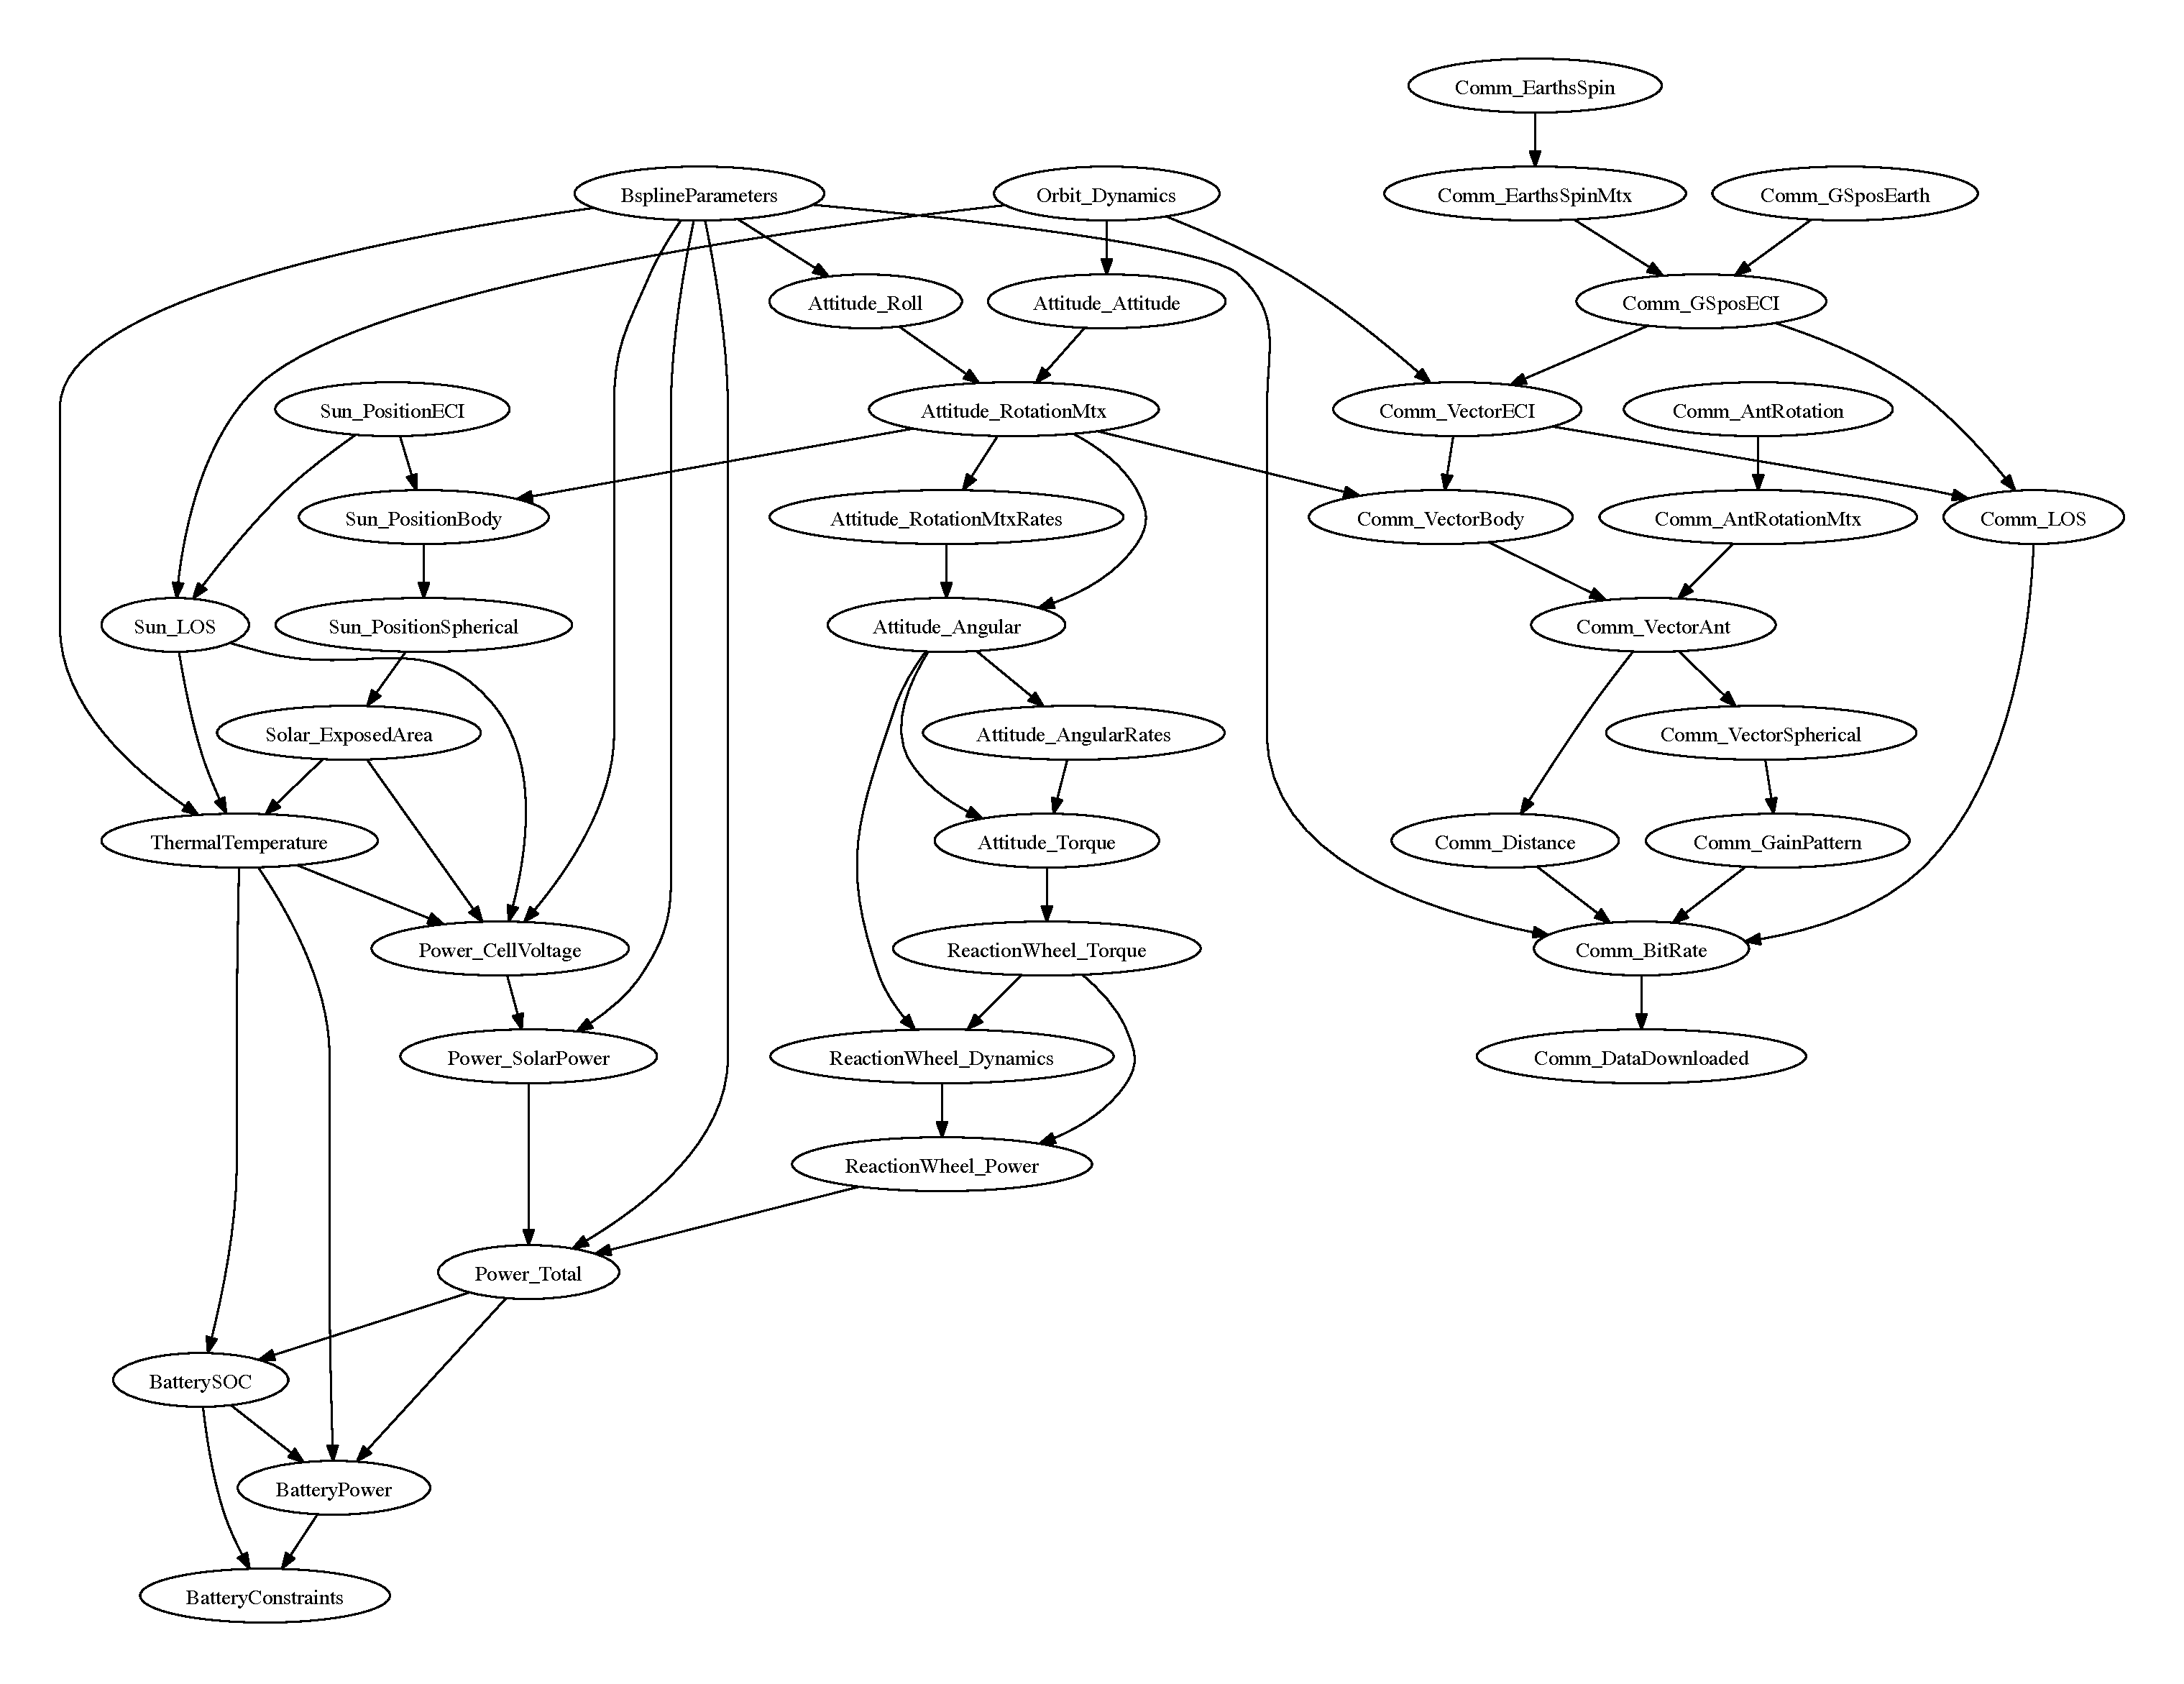
\includegraphics[width=1.1\textwidth]{images/CADRE.pdf}
      \caption{ Dependency graph for the satellite problem. \label{fig:cadre_graph}}
    \end{center}\end{figure}

    \subsection{Results}

        \subsection{Optimization Results}

        The OpenMDAO implementation of the satellite problem was executed on a
        Macbook Pro (2.3 Ghz Core i7 processor, 4GB 1600 Mhz DDR3 memory, running OSX 10.8.5)
        over the course of two days, to a termination tolerance of $10^{-5}$. This tolerance
        was achieved within approximately 106 iterations, using the SNOPT\cite{gill2005snopt}
        optimizer.

        \begin{figure}
        \centering
        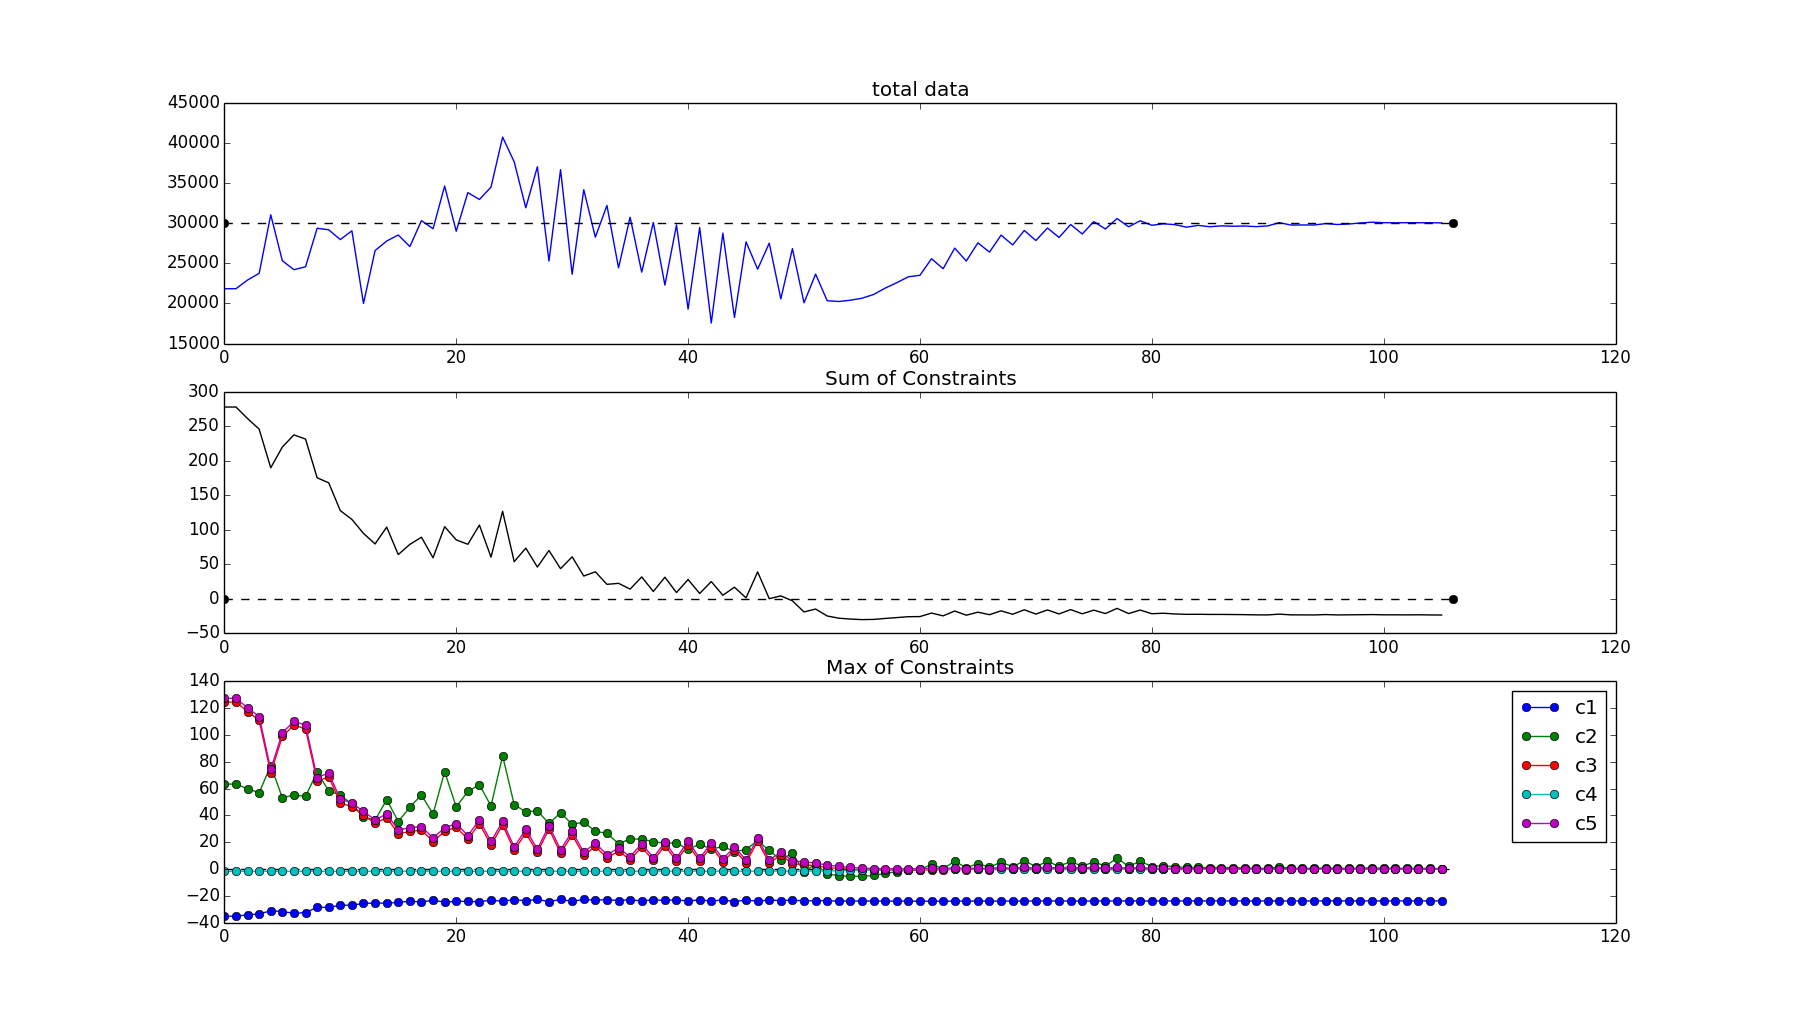
\includegraphics[width=0.99\textwidth]{images/opt}
        \caption[width=0.22\textwidth]{Convergence of the satellite problem.
        \label{convergence}
        }
        \end{figure}


        Figure \ref{convergence} illustrates the convergence of the satellite problem over the course of
        these iterations. The first row plots the
        value of the objective function, the total data downloaded over each design point. The objective
        function oscillated greatly over the course of the first half of the computed iterations, but
        stabilized by the 80th iteration near the value previously determined \cite{CADRE2012}
        to be the optimal design.

        The second row plots the maximum value of each constraint across all design points at
        each iteration. As all of the problem constraint are non-positive for a feasible design,
        this can be taken as a cursory measure of overall problem feasibility.
        The third row plots the maximum value of each constraint across each of the design points,
        but separated according to specific constraint type. These two plots both indicate that the
        oscillatory behavior of the objective function coincided with a steady decrease in design
        infeasibility. Once a feasible state was reached (near the 50th iteration), the optimizer
        began refining the design towards a more favorable value of the objective function.

        \begin{figure}
        \centering
        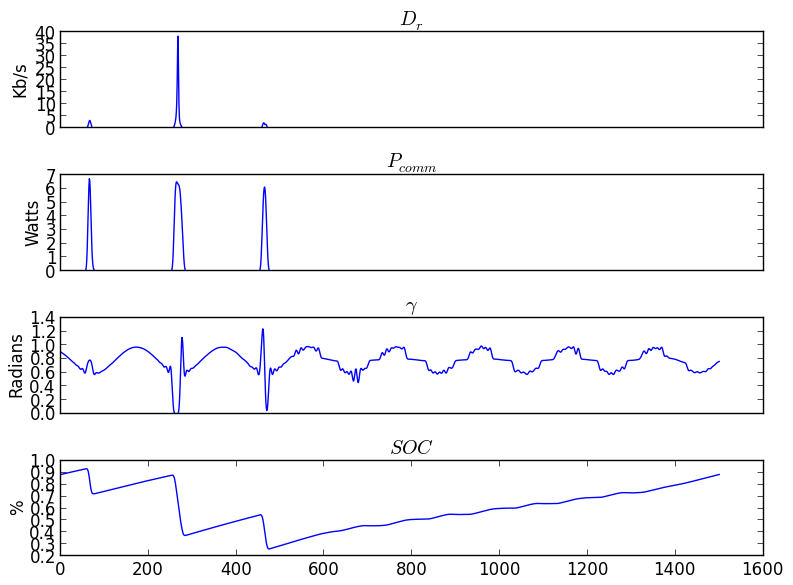
\includegraphics[width=0.8\textwidth]{images/pt_3_data}
        \caption[width=0.4\textwidth]{Plots of the bit rate, communications systems power, craft roll angle,
        and battery charge level over the half-day time period covered by the $4^{\textrm{th}}$ design point.
        \label{pt3_data_results}
        }
        \end{figure}

        Figure \ref{pt3_data_results} shows plots of selected variables for the $4^{\textrm{th}}$ design point,
        to illustrate the fidelity of the recovered solution. These variables are the communications
        bit rate ($D_r$), communications systems power level ($P_{comm}$), craft roll angle ($\gamma$),
        and battery charge level ($SOC$). Prior to the optimization, these variables
        were each instantiated to uniform values
        (across all time points) of 0, 0, $\frac{\pi}{4}$, and 0 respectively. The optimizer, operating on
        OpenMDAO's graph formulation of the problem succeeded at converging each of these variables to the values
        shown, for each time point. Line of sight is seen to have been achieved in three short ranges of time near the
        beginning of the modeled half-day design point. Interestingly, though the data rate achieved in the second
        time period with affirmative line of sight is significantly higher than the other two periods, the optimizer
        converged to a solution that provided power to the communications system near uniformly for each of these
        three time periods. This is likely due to the battery discharge rate and SOC constraints limiting
        the power which may be delivered to the communications system.

        Figure \ref{pt3_data_results} shows that the craft roll angle, $\gamma$, roughly approximates a sine function
        with a wavelength of 90 minutes (the approximate orbital period of the satellite),
        with short term perturbations during the time
        periods where line of sight is gained with the ground station. That is, the optimizer successfully
        converged to a solution with the satellite continuously turned to maximize exposure to the sun,
        except when turning to point its antenna towards the ground station during times when
        communication is possible. This dynamic is also reflected in the battery state of charge ($SOC$)
        data plotting in the bottom row, with the battery losing charge quickly during
        communication with the ground station, but recharging while tracking with the sun.

        Further post processing of the data included automatic geographical rendering of the trajectories of
        the  satellite for each of the 6 design points, using the Google
        Maps\footnote{http://developers.google.com/maps/} and Google
        Earth\footnote{http://developers.google.com/earth/} APIs. The trajectories are
        represented as polygonal chain ("polyline") elements, colored according to the
        satellites communication bit rate with the ground station during the corresponding
        window of time. Each colored line segment are centered on the locations
        determined by the time points when the data bit rate values were calculated
        by the OpenMDAO model.

        Figure \ref{pt3_g_earth} shows the communications bit rate along the trajectories of the
        satellite during the $4^{\textrm{th}}$ design point. This can be compared
        directly with Figure \ref{pt3_data_results}, where one large spike in communications
        bit rate was preceded and then succeeded by two short time periods of lesser
        data rates. Plotted geographically, this is seen to be due to the procession of
        the satellites orbit, where the period of maximal data rate corresponds to a
        pass of the satellite directly over the ground station location. The proceeding and
        succeeding data rate spikes correspond to passes over the near Atlantic and
        Rocky Mountain regions, respectively.


        Figure \ref{allpt_flatmap} similarly shows trajectory and bit rate data plotted
        from all six design points, centered on the United States. The orbital passes
        that are close enough to the ground station for communications can all be seen.
        Figure \ref{allpt_g_earth} zooms this view out to show coverage of the trajectories
        of all design points across the Earth.


        \begin{figure}
        \centering
        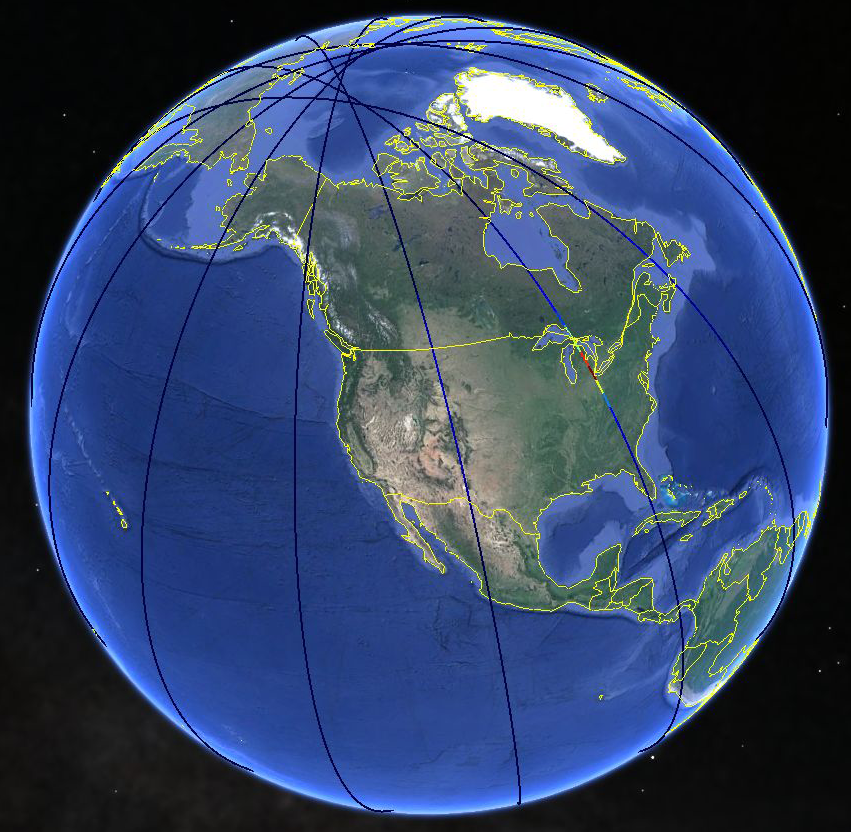
\includegraphics[width=0.8\textwidth]{images/pt3_gearth3}
        \caption[width=0.4\textwidth]{Plot of the trajectories of the satellite
        for the $4^{\textrm{th}}$ design point onto the surface of the Earth, illustrating the
        communication data rates near the ground station.
        \label{pt3_g_earth}
        }

        \end{figure}


        \begin{figure}
        \centering
        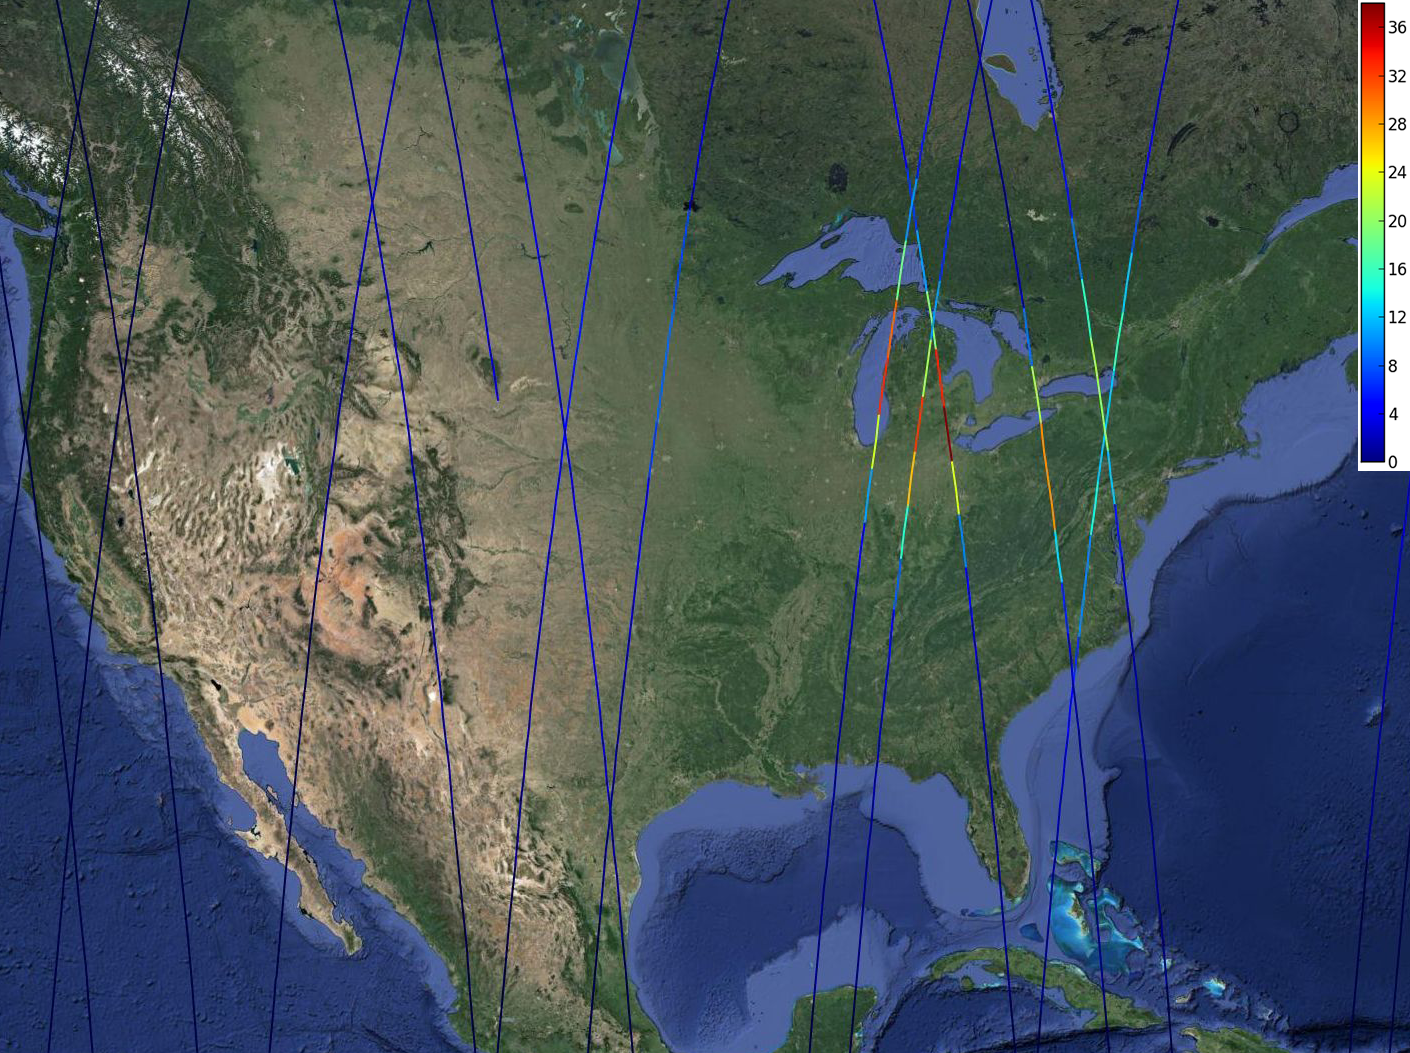
\includegraphics[width=0.8\textwidth]{images/allpts_map_data}
        \caption[width=0.4\textwidth]{Plot of the trajectories of the satellite
        for all 6 design points onto the surface of the Earth, illustrating the
        communication data rates near the ground station.
        \label{allpt_flatmap}
        }

        \end{figure}


        \begin{figure}
        \centering
        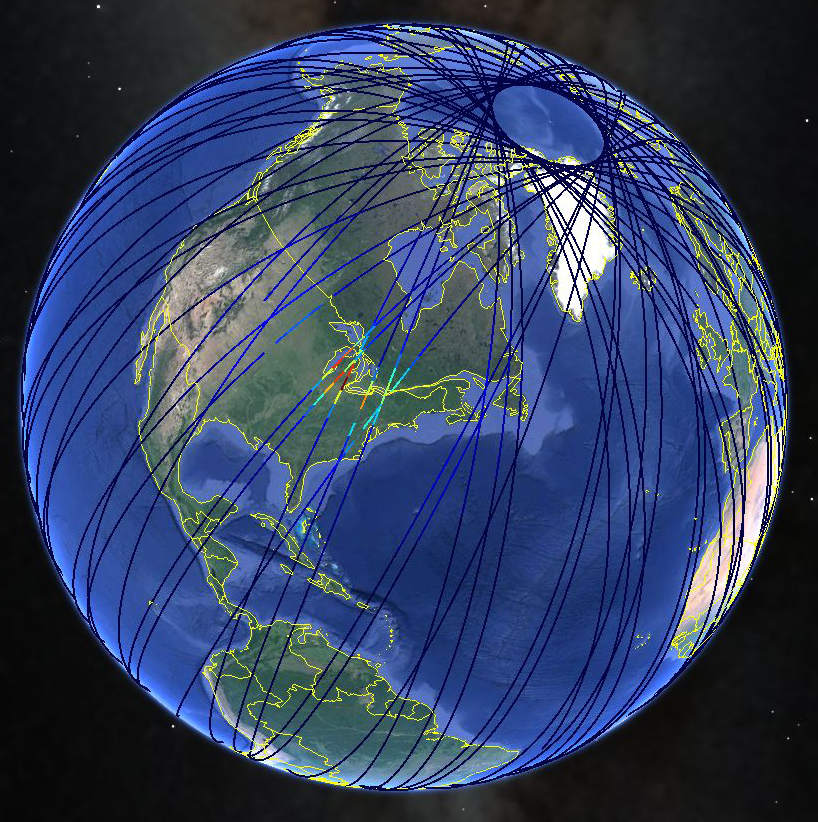
\includegraphics[width=0.8\textwidth]{images/allpts_gearth2}
        \caption[width=0.4\textwidth]{Plot of the trajectories of the satellite
        for all 6 design points onto the surface of the Earth.
        \label{allpt_g_earth}
        }

        \end{figure}

        \subsection{Performance Results}
            Compare size of linear system with and without sparsity. Relative speeds.


  \section{Wind Turbine Design Problem (Justin/Andrew)}

    The goal of this design problem is to perform an aero-structural optimization of 
    a rotor for a horizontal axis wind turbine to maximize its annual energy production. 
    The problem considers the design of the both the rotor and the tower. The structure of
    this problem is much more complex than the small satellite design problem, with 
    nested sub-assemblies of components and more interdisciplinary coupling. However, 
    the problem also has a dramatically smaller design space. 


    \subsection{Problem Formulation}
        The problem formulation is given by: 

        \begin{align}
            \\\txt{max.} &\ \ \sum_{i=1}^6 D_i \notag
            \\\txt{w.r.t.} & \ \ 0 \le I_{setpt} \le 4 \notag
            \\     & \ \ 0 \le P_{comm} \le 25 \notag
            \\     & \ \ 0 \le cellInstd \le 1 \notag
            \\     & \ \ 0 \le finAngle \le \pi/2 \notag
            \\     & \ \ 0 \le antAngle \le \pi \notag
            \\     & \ \ 0.2 \le iSOC \le 1 \notag
            \\\txt{s.t.} & \ \ I_{bat} - 5 \le 0 \notag
            \\     & \ \ -10 - I_{bat} \le 0 \notag
            \\     & \ \ 0.2 - SOC \le 0 \notag
            \\     & \ \ SOC - 1 \le 0 \notag
            \\     & \ \ fSOC - iSOC = 0 \notag
            \label{eqn:wt_formulation}
        \end{align}

        The problem has XX design variables, 1 objective, and YY constraints. Since there are more 
        quantities of interest than design variables, this problem called for forward derivatives calculations. 
        The lower number of design variables make it feasible to solve this problem 
        with finite difference gradients. 


        % \begin{itemize}
        %     \item Design variables, objectives, constraints.
        %     \item this problem uses forward
        %     \item mixed analytic and FD gradients
        %     \item non-relevant, but non-differentiable variables
        % \end{itemize}

    \subsection{Results}
        \begin{itemize}
            \item FD vs analytic results
            \item speed issues without directional derivatives
        \end{itemize}


  \section{Conclusion (Justin/Tristan)}

      This work demonstrates how a graph-based approach to problem formulation compliments and enhances the benefits of gradient based
      optimization. The graph provides a proper structure to handle the necessary bookkeeping to automatically implement complex
      problem formulations while making use of analytic gradients. By implementing this graph based approach in OpenMDAO, the framework
      can alleviate the responsibilities for such bookkeeping from the user entirely which dramatically simplifies implementation.

      The two problems examined in this work demonstrate that a single framework can operate efficiently and effectively on a wide range of large-scale problems.

  \bibliography{references}


\end{document}
